\let\lesson\undefined
\newcommand{\lesson}{\phantomlesson{Bài 4.}}


\setcounter{section}{2}
\section{Bài tập trắc nghiệm}
\begin{enumerate}[label=\bfseries Câu \arabic*:]
	\item \mkstar{3}\\
	{Một xe chuyển động thẳng không đổi chiều, $\SI{1}{\hour}$ đầu xe chạy với tốc độ trung bình $\SI{60}{\kilo\meter/\hour}$ và $\SI{3}{\hour}$ sau xe chạy với tốc độ trung bình $\SI{40}{\kilo\meter/\hour}$. Tính tốc độ trung bình của xe trong suốt thời gian chuyển động.
		\begin{mcq}(4)
			\item $\SI{48}{\kilo\meter/\hour}$.
			\item $\SI{40}{\kilo\meter/\hour}$.
			\item $\SI{58}{\kilo\meter/\hour}$.
			\item $\SI{45}{\kilo\meter/\hour}$.
		\end{mcq}
	}
	\hideall{
		\textbf{Đáp án: D.}
	}
	
	\item \mkstar{3}\\
	{Một người đi xe đạp trên $\dfrac{2}{3}$ đoạn đường đầu với tốc độ trung bình $\SI{10}{\kilo\meter/\hour}$ và $\dfrac{1}{3}$ đoạn đường sau với tốc độ trung bình $\SI{20}{\kilo\meter/\hour}$. Tốc độ trung bình của người đi xe đạp trên cả quãng đường là
		\begin{mcq}(4)
			\item $\SI{12}{\kilo\meter/\hour}$.
			\item $\SI{15}{\kilo\meter/\hour}$.
			\item $\SI{17}{\kilo\meter/\hour}$.
			\item $\SI{13.3}{\kilo\meter/\hour}$.
		\end{mcq}
	}
	\hideall{
		\textbf{Đáp án: A.}
	}
\end{enumerate}
\section{Bài tập tự luận}
\begin{enumerate}[label=\bfseries Bài \arabic*:]
	\item \mkstar{2}
	
	
	{
		Hãy tính tốc độ trung bình ra m/s và km/h của nữ vận động viên tại một số giải thi đấu dựa vào bảng:
		\begin{center}
			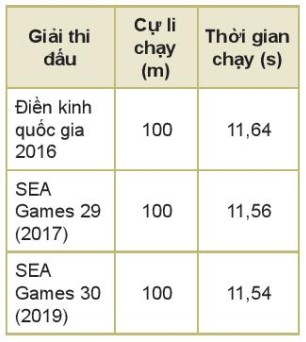
\includegraphics[scale=1]{../figs/VN10-2022-PH-TP005-5.jpg}
		\end{center}
	}
	\hideall
	{
		
		Giải điền kinh quốc  gia 2016 là 100:
		
		$$v_\text{tb} = \dfrac{s}{t} =\dfrac{100}{\SI{11,64}{}} = \SI{8,6}{m/s} = \SI{30,96}{km/h}.$$
		
		SEA GAME 19, 2017  là 100 : 
		
		$$v_\text{tb} = \dfrac{s}{t} =\dfrac{100}{\SI{11,56}{}} = \SI{8,65}{m/s} = \SI{31,141}{km/h}.$$
		
		SEA GAME 30, 2019 là 100: 
		
		$$v_\text{tb} = \dfrac{s}{t} =\dfrac{100}{\SI{11,54}{}}= \SI{8,66}{m/s} = \SI{31,195}{km/h}.$$
	}

	\item \mkstar{2}
	
	
	{
		Một người đi xe máy đi từ ngã tư với tốc độ trung bình $\SI{30}{km/h}$ theo hướng Bắc. Sau 3 phút người đó đến vị trí nào trên hình?
		\begin{center}
			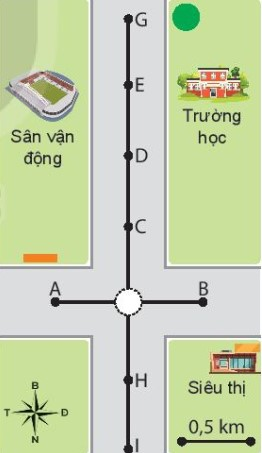
\includegraphics[scale=1]{../figs/VN10-2022-PH-TP005-1.jpg}
		\end{center}
	}
	\hideall
	{
		Sau 3 phút người đó đi được quãng đường là:
		
		$$s = vt = \SI{1,5}{km}.$$ 
		
		Như vậy người đó đến vị trí điểm E.
	}

		\item \mkstar{3}
	
	{
		Hãy tính quãng đường đi được, độ dịch chuyển, tốc độ, vận tốc của bạn A khi đi từ nhà đến trường và khi đi từ trường đến siêu thị. Coi chuyển động của bạn A là chuyển động đều và biết cứ $\SI{100}{m}$ bạn A đi hết $\SI{25}{s}$.
		\begin{center}
			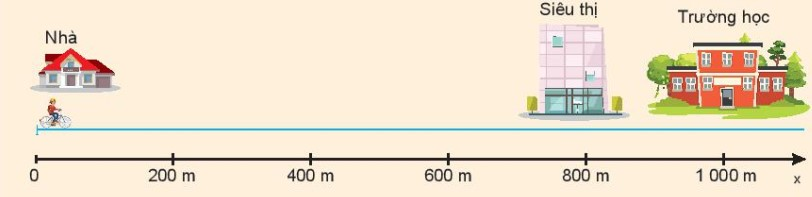
\includegraphics[scale=0.9]{../figs/VN10-2022-PH-TP006-1.jpg}
		\end{center}
	}
	
	\hideall{
		
		Vì bạn A đi từ nhà đến trường là theo 1 hướng, không đổi hướng nên :
		
		Quãng đường đi được và độ dịch chuyển là như nhau và bằng $\SI{1000}{m}$.
		
		Vận tốc và tốc độ là như nhau và bằng : 
		
		$$v = \dfrac{d}{t} =\dfrac{100}{25} = \SI{4}{m/s}.$$
	}
	

	\item \mkstar{3}\\
	{Một ôtô đi trên quãng đường AB với vận tốc $\SI{54}{km/h}$. Nếu giảm vận tốc đi $\SI{9}{km/h}$ thì ôtô đến B trễ hơn dự định 45 phút. Tính quãng đường AB và thời gian dự tính để đi quãng đường đó.
	}
	\hideall{Gọi $t_1$ là thời gian dự định, $v$ là vận tốc ban đầu và $s$ là chiều dài quãng đường AB. Phương trình chuyển động cho các trường hợp đi đúng vận tốc dự kiến và đi chậm hơn lần lượt là 
		\begin{align*}
			s&=vt=54t\\
			s&=(v-9)(t+\SI{0.75}{})=45(t+\SI{0.75}{})
		\end{align*}
		
		Vế trái của hai phương trình giống nhau nên ta cho hai vế phải của hai phương trình bằng nhau, giải được $t_1 =\SI{3,75}{\hour}$.	
		
	}
	
	\item \mkstar{3}
	
	{
		
		Một người đi xe máy chuyển động theo 3 giai đoạn: Giai đoạn 1 chuyển động thẳng đều với 
		$v_1 = \SI{30}{km/h}$ trong $\SI{10}{km}$ đầu tiên; giai đoạn 2 chuyển động với $v_2 = \SI{40}{km/h}$ trong 30 phút; giai đoạn 3 chuyển động trên $\SI{4}{km}$ trong 10 phút. Tính tốc độ trung bình trên cả đoạn đường.
	}
	\hideall{
		
		Thời gian xe máy chuyển động giai đoạn đầu
		
		$$t_1 = \dfrac{s_1}{v_1} = \dfrac{1}{3}\ \text{h}.$$
		
		Quãng đường giai đoạn sau:
		
		$$s_2 = v_2t_2 = \SI{20}{km}.$$
		
		Ta có:
		
		$$s = s_1 + s_2 + s_3 = \SI{34}{km}.$$
		
		$$t = t_1 + t_2 + t_3 = \SI{1}{h}.$$
		
		Vận tốc trung bình:
		
		$$v_\text{tb} = \dfrac{s}{t} = \SI{34}{km/h}.$$
		
	}
	\item \mkstar{3}
	
	{
		Một xe máy điện đi nửa đoạn đường đầu tiên với tốc độ trung bình $v_1 = \SI{24}{km/h}$ và nửa đoạn đường sau với tốc độ trung bình $v_2 = \SI{40}{km/h}$. Tính tốc độ trung bình trên cả đoạn đường.
		
	}
	\hideall{
		
		Thời gian đi nửa đoạn đường đầu:
		
		$$t_1 = \dfrac{S_1}{v_1} = \dfrac{S}{48}.$$
		
		Thời gian đi nửa đoạn đường cuối:
		
		$$t_2 = \dfrac{S_2}{v_2} = \dfrac{S}{80}.$$
		
		Tốc độ trung bình:
		
		$$v = \dfrac{S}{t_1 + t_2} = \dfrac{S}{\dfrac{S}{48} + \dfrac{S}{80}} = \SI{30}{km/h}.$$
		
	}
	\item \mkstar{3}
	
	{
		
		Một ô tô chuyển động trên đoạn đường AB. Nửa quãng đường đầu ô tô đi với tốc độ $\SI{60}{km/h}$, nửa quãng đường còn lại ô tô đi với nửa thời gian đầu với tốc độ $\SI{40}{km/h}$, nửa thời gian sau đi với vận tốc $\SI{20}{km/h}$. Xác định tốc độ trung bình trên cả quãng đường AB.
	}
	\hideall{
		
		Giai đoạn 1:
		
		$$S_1 = \dfrac{S}{2}$$
		
		$$ t_1 = \dfrac{S_1}{v_1} = \dfrac{S}{2v_1} = \dfrac{S}{120}.$$
		
		Giai đoạn 2:
		
		$$S_2 = v_2t_2 = 40t_2.$$
		
		Giai đoạn 3:
		
		$$S_3 = v_3t_3 = 20t_3.$$
		
		$$t_2 = t_3 \Rightarrow S_3 =20t_2.$$
		
		Theo đề bài ta có:
		
		$$S_2 + S_3 = \dfrac{S}{2} \Rightarrow 40t_2 + 20t_2 = \dfrac{S}{2} \Rightarrow t_2 = t_3 = \dfrac{S}{120}.$$
		
		Vận tốc trung bình của cả quãng đường
		
		$$v = \dfrac{S}{\dfrac{S}{120} + \dfrac{S}{120} + \dfrac{S}{120}} = \SI{40}{km/h}.$$
		
		
		
	}
	\item \mkstar{3}
	
	{
		
		Một ô tô chạy trên đoạn đường thẳng từ A đến B phải mất khoảng thời gian $t$. Trong nửa đầu của khoảng thời gian này ô tô có tốc độ là $\SI{60}{km/h}$. Trong nửa khoảng thời gian cuối ô tô có tốc độ là $\SI{40}{km/h}$. Tính tốc độ trung bình trên cả đoạn AB.
	}
	\hideall{
		
		Trong nửa thời gian đầu:
		
		$$S_1 = v_1t_2 = 30t.$$
		
		Trong nửa thời gian cuối:
		
		$$S_2 = v_2t_2 = 20t.$$
		
		Tốc độ trung bình:
		
		$$v_\text{tb} = \dfrac{S}{t} = \dfrac{S_1 + S_2}{t_1+t_2} = \dfrac{30t + 20t}{t} = \SI{50}{km/h}.$$		
	}
	\item \mkstar{3}
	
	{
		
		Một chiếc thuyền cao tốc đi từ bến A đến bến B. Trong $\dfrac{2}{3}$ thời gian đầu tốc độ của thuyền là $v_1 = \SI{45}{km/h}$, thời gian còn lại thuyền chuyển động với tốc độ $v_2$ bằng bao nhiêu để tốc độ trung bình của nó trên cả quãng đường AB là $v = \SI{48}{km/h}$?
		
	}
	\hideall{
		
		- Gọi $t$ (giờ) là tổng thời gian thuyền đi từ bến A đến B, $v$ (km/h) là vận tốc trung bình của thuyền khi đi từ A đến B.
		
		- Khoảng cách giữa hai bến A, B là:
		
		$$S = vt = 48t\ (1).$$
		
		- Theo bài ta có:
		
		$$S = v_1 \dfrac{2t}{3} + v_2 \dfrac{t}{3} = 30t + v_2\dfrac{t}{3}.\ (3)$$
		
		Ta có:
		
		$$48t = 30t + v_2 \dfrac{t}{3} \Rightarrow v_2\dfrac{t}{3} = 18t \Rightarrow v_2 = \SI{54}{km/h}.$$
	}
	\item \mkstar{3}
	
	{
		Một cậu bé dắt chó đi dạo về nhà, khi còn cách nhà $\SI{10}{m}$, con chó chạy về nhà với tốc độ $\SI{5}{m/s}$. Vừa đến nhà nó lại chạy ngay lại với tốc độ $\SI{3}{m/s}$. Tính tốc độ trung bình của chú chó trong quãng đường đi được kể từ lúc chạy về nhà đến lúc gặp lại cậu bé, biết cậu bé đi đều với tốc độ $\SI{1}{m/s}$.
	}
	\hideall{
		
		Thời gian chú chó về đến nhà là
		
		$$t_1 = \dfrac{S}{v_1} = \SI{2}{s}.$$
		
		Trong thời gian đó cậu bé đi được
		
		$$S_1 = t_1 v = 1 \cdot 2 = \SI{2}{m}.$$
		
		Khoảng cách từ cậu bé đến nhà lúc đó là
		
		$$S_2 = S - S_1 = \SI{8}{m}.$$
		
		Thời gian chú chó chạy từ nhà tới lúc gặp lại cậu bé
		
		$$t_2 = \dfrac{S_2}{v_2 + v} = \SI{2}{s}.$$
		
		Chú chó đã quay lại một đoạn là:
		
		$$S_2 = v_2t_2 = 3 \cdot 2 = \SI{6}{m}.$$
		
		Tổng thời gian $t = \SI{4}{s}$, tổng quãng đường là 
		
		$$S = 10 + 6 = \SI{16}{m}.$$
		
		Tốc độ trung bình của chú chó trong cả quá trình là: 
		
		$$v_\text{tb} = \dfrac{S + S_2}{t_1 + t_2} = \SI{4}{m/s}.$$
	}
	\item \mkstar{3}
	
	{
		Một ôtô chuyển động trên đoạn đường MN. Trong một phần hai quãng đường đầu đi với $v = \SI{40}{km/h}$. Trong một phần hai quãng đường còn lại đi trong một phần hai thời gian đầu với $v = \SI{75}{km/h}$ và trong một phần hai thời gian cuối đi với $v = \SI{45}{km/h}$. Tính tốc độ trung bình trên đoạn MN.
	}
	\hideall{
		
		Ta có: $s_1 = \dfrac{S}{2}$, mà $s_1 = v_1t_1 = 40t_1 \Rightarrow t_1 = \dfrac{S}{80}.$
		
		Theo đề bài:
		
		$$s_2 = s_3 + s_4 = 75\left(\dfrac{t-t_1}{2}\right) + 45\left(\dfrac{t-t_1}{2}\right) = 60t - \dfrac{60S}{80}.$$
		
		Mặt khác:
		
		$$S = s_1 + s_2 = \dfrac{S}{2} + 60t - \dfrac{60S}{80} \Leftrightarrow \text{1,25S} = 60t \Rightarrow S = 48t.$$
		
		Tốc độ trung bình trên đoạn MN
		
		$$v_\text{tb} = \dfrac{S}{t} = \SI{48}{km/h}.$$
		
	}
	\item \mkstar{3}
	
	{
		
		Một người đua xe đạp đi trên $\dfrac{1}{3}$ quãng đường đầu với $\SI{25}{km/h}$. Tính tốc độ của người đó đi trên đoạn đường còn lại. Biết rằng $v_\text{tb} = \SI{20}{km/h}$.
	}
	\hideall{
		
		Ta có:
		
		$$S_1 = v_1t_1 \Rightarrow t_1 = \dfrac{S_1}{v_1} = \dfrac{S}{75}.$$
		
		$$S_2 = v_2t_2 \Rightarrow t_2 = \dfrac{S_2}{v_2} = \dfrac{2S}{3v_2}.$$
		
		Lại có:
		
		$$v_\text{tb} = \dfrac{S}{t} = \dfrac{S}{t_1+t_2} = \SI{20}{km/h} \Rightarrow \dfrac{S}{\dfrac{S}{75} + \dfrac{2S}{3v_2}} = \SI{20}{km/h}$$
		
		$$\Rightarrow 225 v_2 = 60 v_2 + 3000 \Rightarrow v_2 = \SI{18,182}{km/h}.$$
	}
	\item \mkstar{3}
	
	{
		
		Một người đi xe máy trên một đoạn đường thẳng AB. Trên một phần ba đoạn đường đầu đi với $v_1 = \SI{30}{km/h}$, một phần ba đoạn đường tiếp theo với $v_2 = \SI{36}{km/h}$ và một phần ba đoạn đường cuối cùng đi với $v_3= \SI{48}{km/h}$. Tính $v_\text{tb}$ trên cả đoạn AB.
		
	}
	\hideall{
		
		Trong một phần ba đoạn đường đầu:
		
		$$S_1 = v_1 t_1 \Rightarrow t_1 = \dfrac{S_1}{v_1} = \dfrac{S}{3v_1}.$$
		
		Tương tự: 
		
		$$t_2 = \dfrac{S_2}{v_2} = \dfrac{S}{3v_2}; t_3 = \dfrac{S_3}{v_3} = \dfrac{S}{3v_3}.$$
		
		$v_\text{tb}$ trên cả đoạn AB
		
		$$v_\text{tb} = \dfrac{S}{t_1 + t_2 + t_3} = \SI{36,62}{km/h}.$$
		
	}
	\item \mkstar{3}
	
	{
		
		Một người đi xe bắt đầu cho xe chạy trên đoạn đường thẳng: trong 10 giây đầu xe chạy được quãng đường $\SI{50}{m}$, trong 10 giây tiếp theo xe chạy được $\SI{150}{m}$. Tính tốc độ trung bình của xe máy trong khoảng thời gian nói trên.
	}
	\hideall{
		
		Tốc độ trung bình của xe máy
		
		$$v_\text{tb} = \dfrac{S_1 + S_2}{t_1 + t_2} = \SI{10}{m/s}.$$
	}
	\item \mkstar{3}
	
	{
		
		Một người đi xe đạp từ A đến B với tốc độ $\SI{12}{km/h}$ trong $\dfrac{1}{3}$ quãng đường, và tốc độ $\SI{18}{km/h}$ trong $\dfrac{2}{3}$ quãng đường còn lại. Tính tốc độ trung bình của người đó trên cả đoạn đường AB.
	}
	\hideall{
		
		Thời gian đi $\dfrac{1}{3}$ quãng đường đầu:
		
		$$t_1 = \dfrac{S}{3v_1} = \dfrac{S}{36}.$$
		
		Thời gian đi $\dfrac{2}{3}$ quãng đường còn lại:
		
		$$t_2 = \dfrac{2S}{3v_2} = \dfrac{S}{27}.$$
		
		Tốc độ trung bình của người đó
		
		$$v_\text{tb} = \dfrac{S}{t_1 + t_2} = \dfrac{S}{\dfrac{S}{36} + \dfrac{S}{27}} \approx \SI{15,43}{km/h}.$$
	}
	\item \mkstar{3}
	
	{
		
		Một xe chuyển động thẳng không đổi chiều có vận tốc trung bình là $\SI{20}{km/h}$ trên $\dfrac{1}{4}$ đoạn đường đầu và $\SI{40}{km/h}$ trên $\dfrac{3}{4}$ đoạn đường còn lại. Tìm tốc độ trung bình của xe trên cả đoạn đường.
	}
	\hideall{
		
		Thời gian đi $\dfrac{1}{4}$ quãng đường đầu:
		
		$$t_1 = \dfrac{S}{4v_1}.$$
		
		Thời gian đi $\dfrac{3}{4}$ quãng đường còn lại:
		
		$$t_2 = \dfrac{3S}{4v_2}.$$
		
		Tốc độ trung bình của người đó
		
		$$v_\text{tb} = \dfrac{S}{t_1 + t_2} =  \SI{32}{km/h}.$$
	}
	\item \mkstar{3}
	
	{
		
		Một xe chuyển động thẳng không đổi chiều, trong nửa thời gian đầu xe chạy với vận tốc $\SI{12}{km/h}$. Trong nửa thời gian sau xe chạy với vận tốc $\SI{18}{km/h}$. Tính tốc độ trung bình trong suốt thời gian đi.
	}
	\hideall{
		
		Trong nửa thời gian đầu
		
		$$s_1  = v_1 t_1 = \dfrac{t}{2} v_1.$$
		
		Trong nửa thời gian sau
		
		$$s_2  = v_2 t_2 = \dfrac{t}{2} v_2.$$
		
		Tốc độ trung bình trong suốt thời gian
		
		$$v_\text{tb} = \dfrac{s_1 + s_2}{t} = \SI{15}{km/h}.$$
	}
	\item \mkstar{3}
	
	{
		
		Một ô tô chạy liên tục, trong 2 giờ đầu với tốc độ $\SI{80}{km/h}$, trong 1 giờ sau chạy với tốc độ $\SI{50}{km/h}$. Tốc độ trung bình của xe trong cả quá trình là bao nhiêu?
	}
	\hideall{
		
		Đoạn đường đi được trong 2 giờ đầu
		
		$$s_1 = v_1 t_1.$$
		
		Đoạn đường đi được trong 1 giờ sau
		
		$$s_2 = v_2t_2.$$
		
		Tốc độ trung bình của xe
		
		$$v_\text{tb} = \dfrac{s_1 + s_2}{t_1 + t_2} = \SI{70}{km/h}.$$
		
	}
\end{enumerate}